\documentclass[12pt,letterpaper,titlepage]{article}

\usepackage{fontspec}
\defaultfontfeatures{Mapping=tex-text}
\usepackage{xunicode}
\usepackage{xltxtra}
\usepackage{amsmath}
\usepackage{pdfpages}
\usepackage{amsfonts}
\usepackage{amssymb}
\setcounter{secnumdepth}{0}
\usepackage{nameref}
\usepackage{enumitem}
\usepackage{environ}
\usepackage{pgfplots}

\setmainfont{Times New Roman}
\showboxdepth=\maxdimen
\showboxbreadth=\maxdimen


\usepackage{paracol}
\usepackage{wrapfig}
\globalcounter{table}
\globalcounter{figure}
\usepackage{graphicx}
\usepackage[left=1in,right=1in,top=1in,bottom=1in]{geometry}
\graphicspath{{img/}}

\author{Jacob Abel}
\title{	Homework 1
	\\\large ECE3544 CRN:82989
}

\setlength{\parskip}{0.5em}

\begin{document}
\maketitle
\begin{raggedright}

\paragraph{Problem 1: }
Using 2's complement arithmetic, add the following decimal numbers, showing all work. i.e. perform $17+19$. Use the smallest number of bits possible to represent each number and the sum without overflow. 

\begin{align*}
17+19 &=
\end{align*}

\paragraph{Problem 2: }
For the addition in problem 1, use one less bit to represent the numbers and show how the overflow can be detected.

\paragraph{Problem 3: }
Using the same guidelines as for problem 1, subtract decimal $87$ from $37$, i.e. perform $37-87$.

\paragraph{Problem 4: }
Give the hexadecimal representation of the answer to problem 3.

\paragraph{Problem 5: }
Write the truth table and Boolean function implemented by the CMOS gate below.

\begin{center}
\begin{paracol}{3}
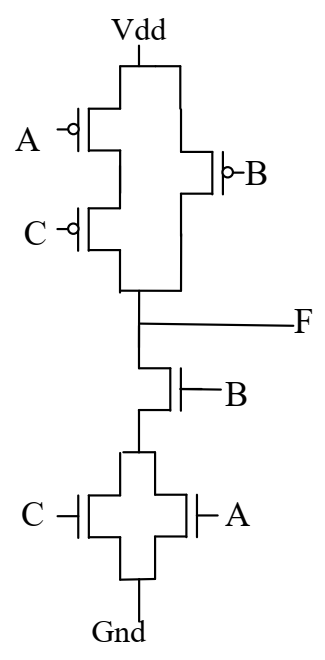
\includegraphics[width=\textwidth, height=17\baselineskip, keepaspectratio=true]{hw1q5}
\switchcolumn
\begin{tabular}{|ccc|c|}
\hline
   A & B & C & F 
\\\hline
   0 & 0 & 0 &   
\\ 0 & 0 & 1 &   
\\ 0 & 0 & 0 &   
\\ 0 & 0 & 1 &   
\\ 0 & 1 & 0 &   
\\ 0 & 1 & 1 &   
\\ 0 & 1 & 0 &   
\\ 0 & 1 & 1 &   
\\ 1 & 0 & 0 &   
\\ 1 & 0 & 1 &   
\\ 1 & 0 & 0 &   
\\ 1 & 0 & 1 &   
\\ 1 & 1 & 0 &   
\\ 1 & 1 & 1 &   
\\ 1 & 1 & 0 &   
\\ 1 & 1 & 1 &   
\\\hline

\end{tabular}
\end{paracol}
\end{center}

\paragraph{Problem 6: }
Draw transistor schematics of a CMOS gate for each of the following Boolean functions:
\begin{enumerate}[label=\alph*)]
\item $F=\overline{(W+Z)\cdot(Y+X)}$
\item $G=\overline{(B+C+D)\cdot A}$
\end{enumerate}

\paragraph{Problem 7: }
Which would you expect to have a bigger effect on the power consumed by a CMOS circuit, a $5\%$ increase in the power supply voltage ($V_{dd}$)or a $10\%$ increase in total capacitance?Briefly explain your answer.

\end{raggedright}
\end{document}
